\subsection{Problem Formulation}
Given:
\begin{itemize}
	\item A directed graph $G = (V, E)$
	\item A capacity function $c: E \rightarrow \mathbb{Z}^+$
	\item A source $s$ and a sink $t$.
\end{itemize}
Find:
\begin{itemize}
	\item A flow $f: E \rightarrow \mathbb{R}$ such that
		\begin{itemize}
			\item Capacity constraints: $\forall e \in E, ~f(e) \le c(e)$.
			\item Non-negativity: $\forall e \in E, ~f(e) \ge 0$.
			\item Conservation constrains: $\forall v \in V - \{s, t\}, ~\sum_{(u,v) \in E} f(u,v) = \sum_{(v, u) \in E}f(v,u)$
		\end{itemize}
	\item To maximize net flow out of $s$:
	\[|f| = \sum_{(s,u) \in E} f(s, u) - \sum_{(u,s) \in E} f(u,s)\]
\end{itemize}
The following is an example of network flow:
\begin{figure}[H]
	\centering
	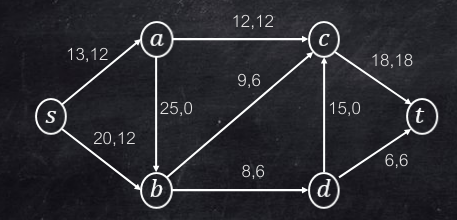
\includegraphics[width=0.5\textwidth]{fig/flow.png}
\end{figure}
The first number on the edge is the capacity of the edge. The second number is the flow on each edge. The flow value $|f| = 24$.

\subsection{Residual Graph}
After we have built up a flow $f$, we construct a residual graph $G_f$ that shows all the edges on which we can still send flow.

Rules for constructing residual graph:
\begin{itemize}
	\item If $G$ has edge $(u, v)$ with $f(u, v) < c(u, v)$ then $G_f$ has edge $(u, v)$ with capacity $c(u, v) - f(u, v)$. (Excess capacity of $(u,v)$)
	\item If $G$ has edge $(u, v)$ with $f(u, v) > 0$, then $G_f$ has edge $(v, u)$ with capacity $f(u, v)$. (Amount of flow can be removed from $(u,v)$)
\end{itemize}

An example is as following. Note that edges that were ``saturated'' do not exist in forward direction.
\begin{figure}[H]
	\centering
	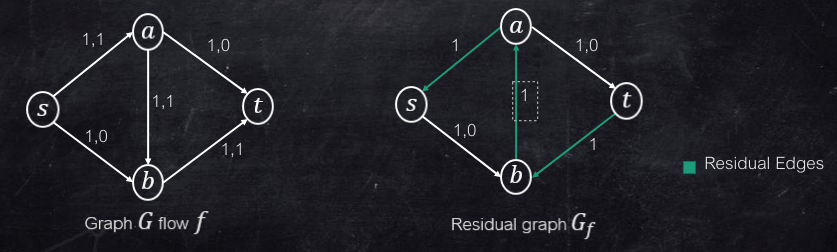
\includegraphics[width=0.6\textwidth]{fig/gf.png}
\end{figure}

\subsection{Adding Two Flow}
If $f_1$ and $f_2$ are two flows, we can add them together to get a flow $f$ as follows:
\begin{itemize}
	\item For an edge $(u,v)$, $f(u,v) = f_1(u,v) + f_2(u,v)$.
	\item If $f_1$ has a positive flow on edge $(u, v)$, and $f_2$ on edge $(v, u)$ in residual graph, then $f(u,v) = f_1(u,v) - f_2(v,u)$.
\end{itemize}
Note that the flows will be non-negative as long as $f_1(u,v) \ge f_2(v, u)$ in second case. It will always be true because we give the edge $(v, u)$ a capacity of $f_1(u, v)$ in $G_{f_1}$.


